\documentclass[../main.tex]{subfiles}
\graphicspath{{\subfix{../images/}}}
\begin{document}

% \subsubsection{Camera Synchronization} \label{time_sync_cam}

Accurate video timestamps are essential for aligning image data with LiDAR point clouds. To achieve frame-level temporal precision, the Minion system embeds timestamps directly into the H.264/H.265 video stream generated by the Jetson Xavier using the GStreamer framework. This ensures that timing information remains synchronized with the frame itself, surviving compression, transmission, and playback.

% \paragraph{prior solution}
% Earlier implementations of the Minion perception system—originally developed by Thompson~\cite{thompson2023} employed a custom GStreamer plugin that performed two timestamping operations.
% First, it generated an adjacent .csv file containing timestamps that aligned to each frame of locally recorded video; second, it embedded the same timestamps into the closed-caption (CEA-608) layer of the \ac{RTSP} video stream.
% While this method was effective for offline data processing using the locally saved video files, the video stream is conducted asynchronously, and the RTSP protocol is unable to keep the closed-caption stream data linked to video frames.
% This limitation motivated the development of an \ac{SEI}-based synchronization method described below.
Earlier implementations of the Minion perception system—originally developed by Thompson~\cite{thompson2023}—employed a custom GStreamer plugin that performed two time-stamping operations. 
First, it generated an adjacent .csv file containing timestamps aligned to each frame of the locally recorded video. 
Second, it embedded the same timestamps into the closed-caption (CEA-608) layer of the \ac{RTSP} video stream. 
While effective for offline data processing using the saved video files, this method was limited by the asynchronous nature of \ac{RTSP}, which cannot maintain a persistent link between closed-caption data and video frames. 
This limitation motivated the development of the \ac{SEI}-based synchronization method described below.

% \paragraph{developed solution}

The current implementation replaces the caption-based approach with direct timestamp embedding using Supplemental Enhancement Information (SEI) Network Abstraction Layer (NAL) units defined in the H.264/H.265 standard.
Each video frame receives a GPS-disciplined system timestamp at the instant of capture from the camera sensor. These timestamps are stored as 64-bit values (milliseconds since Unix epoch) and attached to each frame via a custom GStreamer extension. % (CustomTimestampMeta).
This method keeps the timestamp data inextricably linked to the same video layer that is transmitted over \ac{RTSP}, guaranteeing that each video frame received will have a timestamp, even if dropped frames are experienced.
The complete video processing pipeline is visualized as a block diagram in Appendix \ref{append_video_pipeline}.

% During encoding, a pad probe inserts the SEI NAL units immediately before the RTP payload (rtph264pay), ensuring that every encoded frame carries its own timestamp embedded within the bitstream.
% Because this method fits within the encoding standard, the timestamps persist through compression and streaming, which eliminates the complexity of the prior approach and maintains compatibility with all conventional video decoders.

\begin{figure}[htbp]
\centering
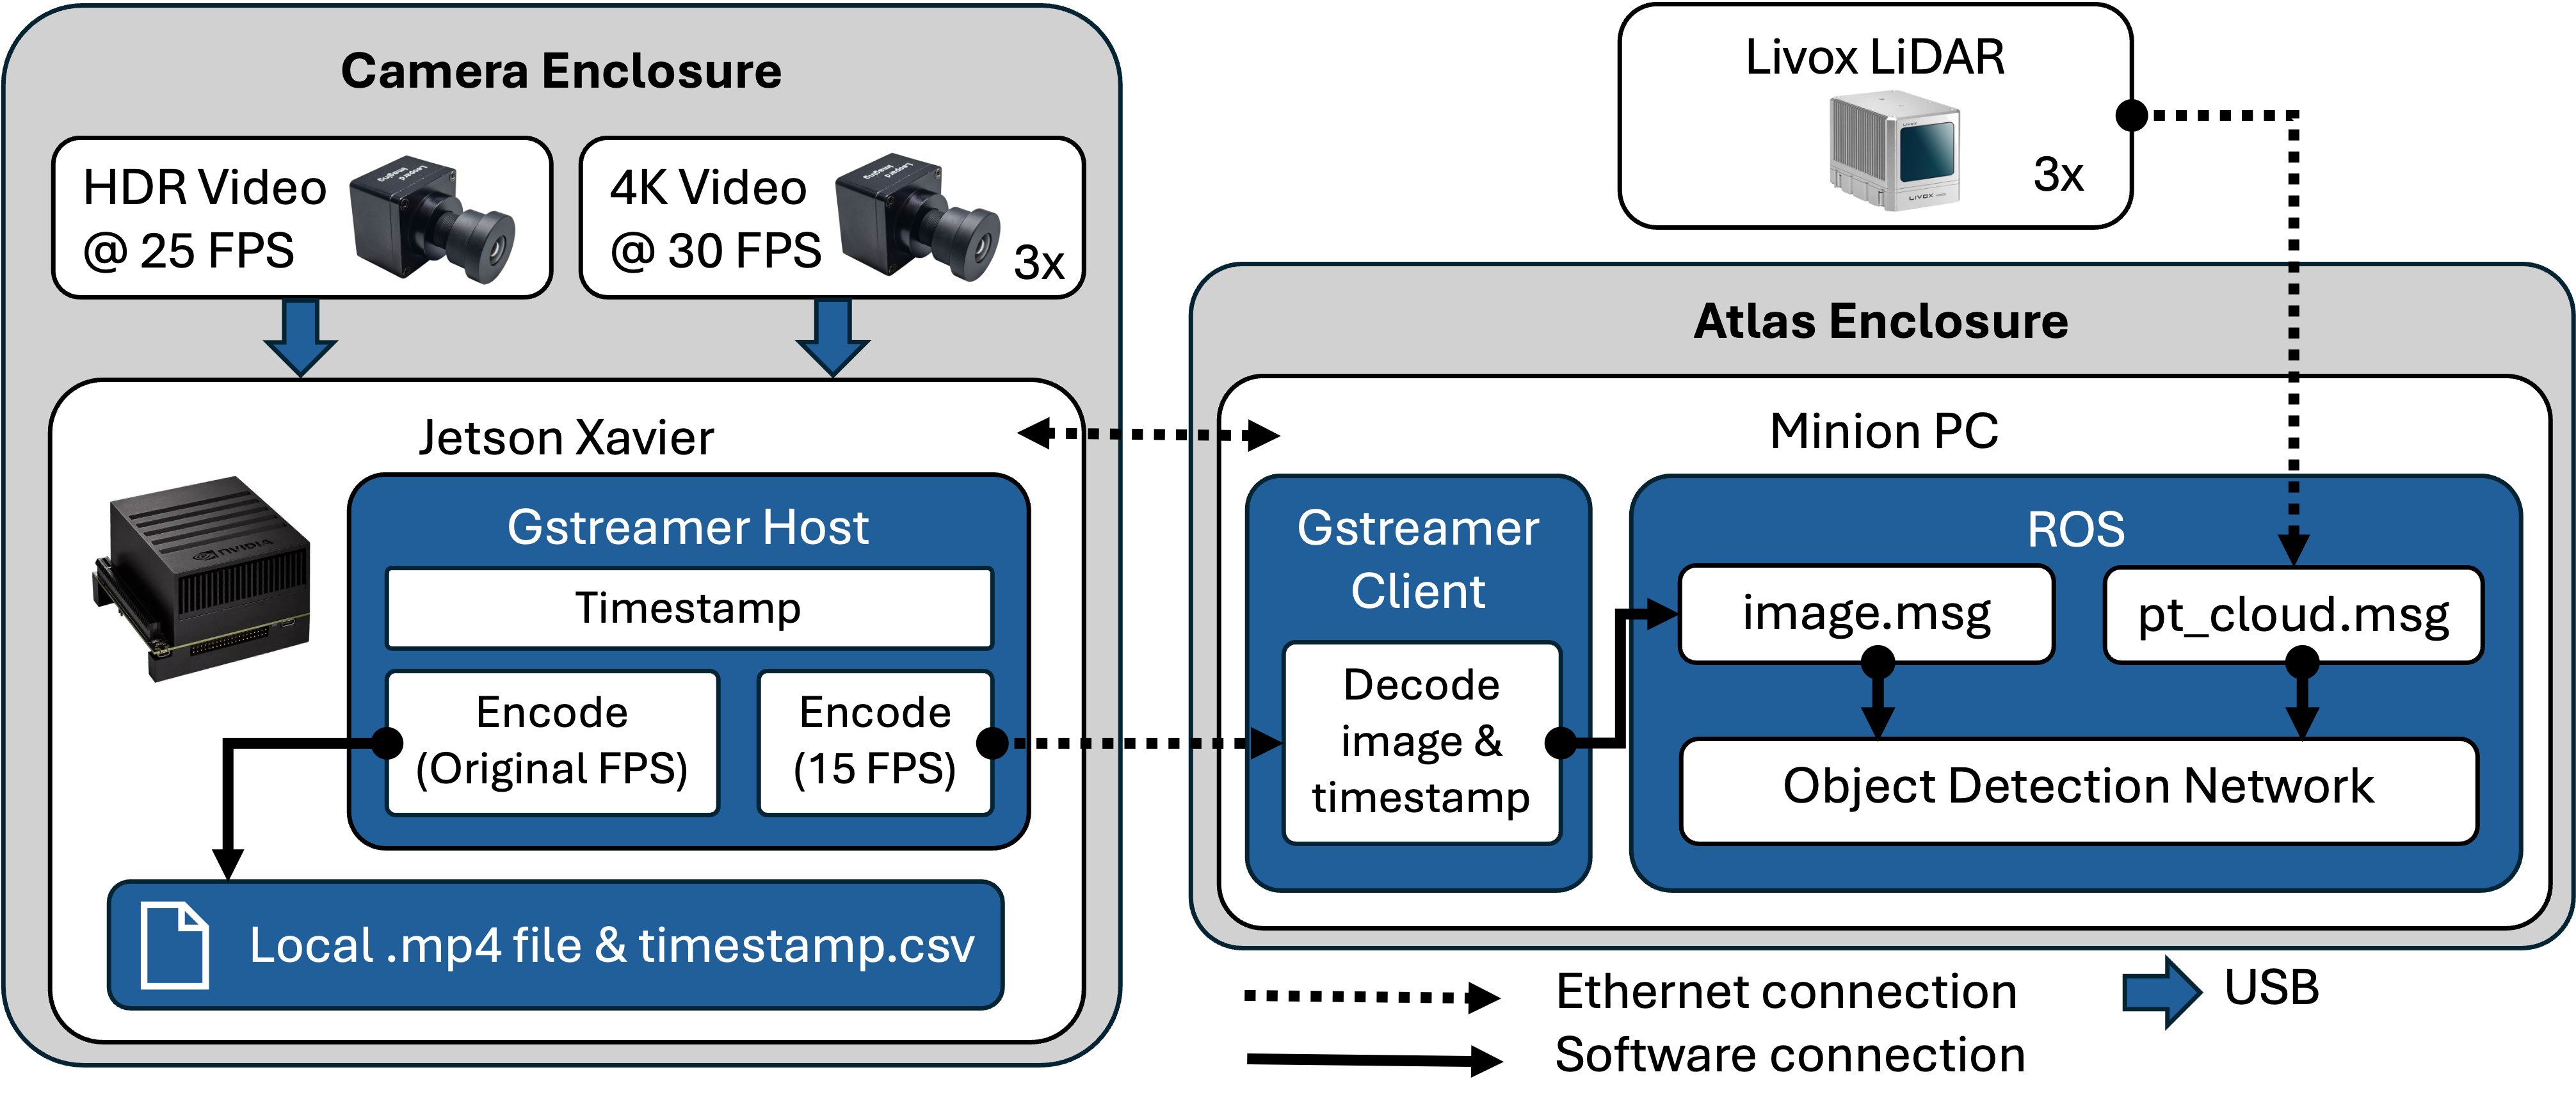
\includegraphics[width=0.8\textwidth]{Images/Block_Diagram.png}
\caption{LAN diagram for Minion USV}
\label{fig:sensor_block_diagram}
\end{figure}



% v4l2src → videoconvert → videorate → x264enc → [SEI insertion] → rtph264pay → RTSP stream

% Captured video at 2880×1860px and 60fps is downsampled to 10fps for transmission, balancing temporal resolution with network bandwidth. The SEI timestamp metadata is attached prior to frame-rate conversion, ensuring that each output frame retains its original capture time.
% The pipeline is fully compliant with ITU-TH.264 Annex~D and has been verified for compatibility with both H.264 and H.265 encoders.

At the receiving end, the Atlas PC decodes incoming streams using a complementary GStreamer pipeline equipped with a pad probe on the \texttt{h264parse} element. This probe identifies SEI NAL units and extracts the embedded timestamp payload before decoding. The recovered timestamps are then written to the ROS message headers of the corresponding image frames via the \texttt{image\_transport} framework.


\begin{figure}[htbp]
\centering
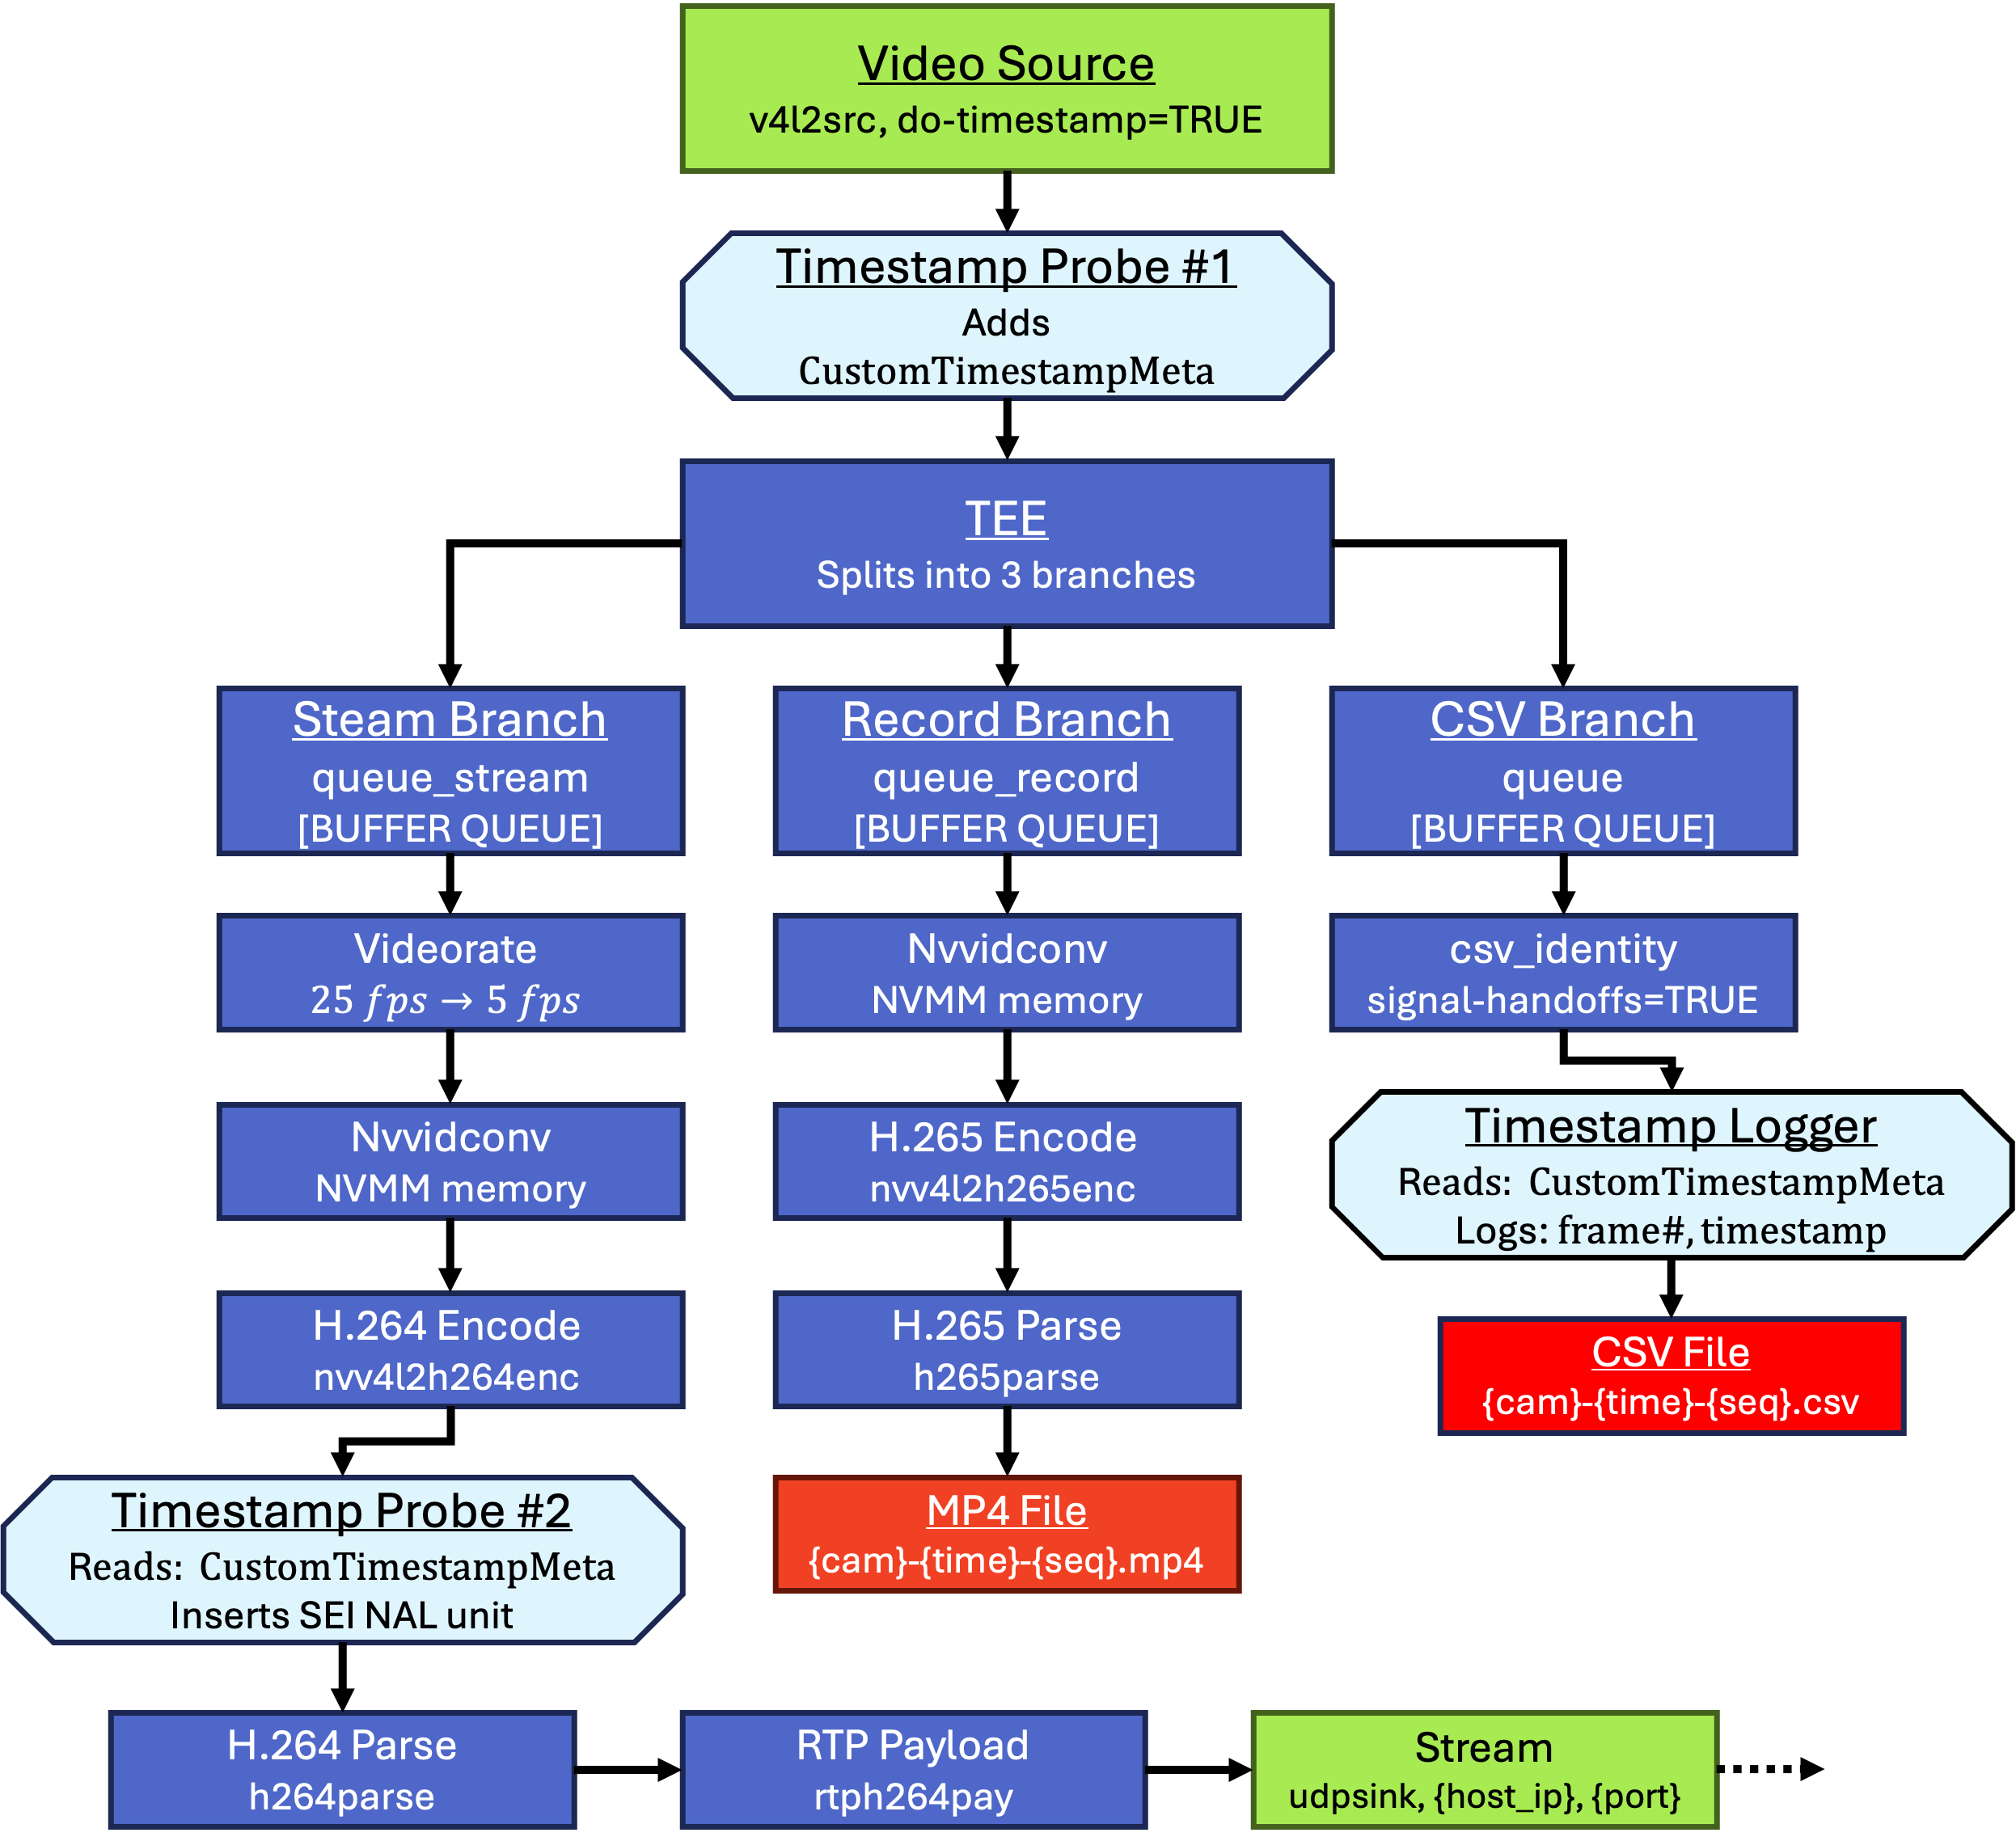
\includegraphics[width=0.95\textwidth]{Images/gstreamer_block.png}
\caption{Block diagram of the NVIDIA Jetson's video pipeline. Green rectangles represent video data entering or leaving the pipeline, while red rectangles indicate local file creation. Light-blue rectangles with chamfered corners denote timestamp acquisition and application operations within the pipeline.}
\label{video_pipeline}
\end{figure}


\end{document}